\documentclass{article}
\usepackage[utf8]{inputenc}
\usepackage{titling}
\usepackage{graphicx}
\usepackage{xcolor}
\usepackage[colorlinks=true,linkcolor=darkgray, urlcolor =gray]{hyperref}
\usepackage[spanish]{babel}
\DeclareUnicodeCharacter{301}{~}
\usepackage{url}
\usepackage{graphicx}
\usepackage{caption}
\usepackage{subcaption}
\DeclareUnicodeCharacter{202F}{\,}
\usepackage{float}


\title{Caso práctico: primera entrega}
\author{Grupo O\\ Álvaro Fernández Palma\\ Alina Altynguzhina\\ Iman Hasnaouia Meskini\\ Cristina Díaz García\\ \\3º de Ingeniería Informática}
\date{Diciembre 2018}

\renewcommand\maketitlehooka{\null\mbox{}\vfill}
\renewcommand\maketitlehookd{\vfill\null}


\begin{document}

\addcontentsline{toc}{section}{Índice general}

\begin{titlingpage}
\maketitle

\end{titlingpage}

\newpage

\tableofcontents

\newpage

\section{Introducción}

\subsection{Descripción de la organización y de su actividad principal} 

La empresa sobre la que vamos a trabajar se llama Puente. La razón por la que la hemos escogido es que uno de nuestros compañeros trabaja allí. Se trata de una empresa que presta servicios a otras empresas respecto a publicidad: creación de marca (branding), storytelling, programación web y tienda online, redes sociales, videos/spots, resumiendo, todo lo relacionado con marketing. Con el objetivo de dar una visibilidad a las empresas de cualquier tamaño y llegar a cualquier público con eficacia. Entre los clientes se encuentran: Adidas, Suzuki, Ubago, Malaga Wagen, etc

\subsection{Breve resumen del trabajo realizado}

Nuestro trabajo consistió en hacer un informe sobre una empresa relacionándolo con todo lo aprendido en las clases.  Se han buscado empresas y propuesto alternativas, y al final se escogió una empresa en la que uno de nuestros miembros del grupo es trabajador. Al principio del trabajo hablamos de conceptos generales y vistos en clase.  

\section{Conceptos generales}

\subsection{Identificar el sistema físico, directivo y de información de la organización. Describirlos desde el punto de vista funcional}

En la empresa elegida, nuestro sistema físico se compone de los siguientes elementos: 

\begin{itemize}
\item El hardware usado para trabajar:  portátiles, ordenadores de sobremesa y todos los periféricos usados en ellos (teclados, pantallas, ratones, auriculares). 
\end{itemize}

El sistema directivo, por otra parte, tiene las siguientes partes: 

\begin{itemize}
\item Reuniones periódicas para decidir cómo actuar ante las diferentes problemáticas que puedan surgir durante el desempeño de las distintas actividades comerciales y de desarrollo. 
\end{itemize}

El sistema de información es, por otra parte:

\begin{itemize}
\item Cada una de los requisitos de las empresas que han solicitado los servicios.
\item Las estadísticas de uso del servicio proporcionado (uso de la página web desarrollada, impacto del ejercicio de márketing realizado...). También los usuarios de estos servicios.
\item Los servidores y documentos en los que se guarda toda la información, tanto de los clientes como de los productos y servicios ofrecidos.
\end{itemize} 

\subsection{Niveles de utilización de los sistemas de información existentes en la organización: operativo/transaccional, táctico y estratégico.}

En la empresa, la gerencia de operaciones la componen cada uno de los trabajadores de rango inferior: programadores, community managers, relaciones humanas, etc.  

La gerencia intermedia son cada uno de los jefes de los diferentes departamentos: el departamento de desarrollo, el de marketing, etc. 

Finalmente, la alta dirección es el jefe y dueño de la empresa.

\section{Infraestructura de TIC}

\subsection{Hardware}

Todos los departamentos están ubicados en la misma sala. Y los departamentos se separan por mesas grandes. Se tienen varias salas: 

Para trabajar: para computación (destinado para todos los departamentos) y para fotografía (para departamento comercial y de diseño)  

Para descansar: zona para comer y descansar.  

Para reuniones: zona habilitada para reunir con los clientes y debatir asuntos.  

Se utilizan los MAC por cada trabajador.

\subsection{Software y otras plataformas}

\begin{center}
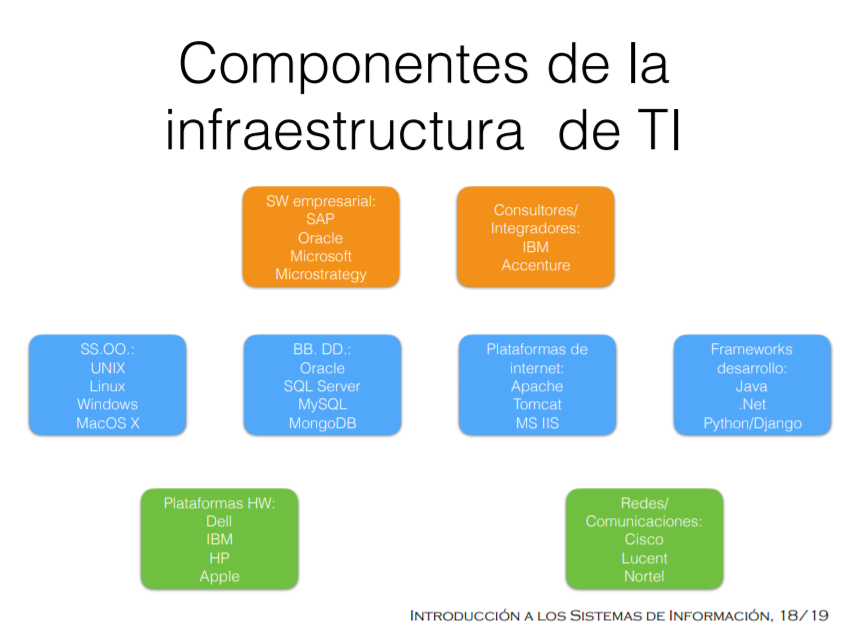
\includegraphics[scale=0.5]{images/componentes.png}
\end{center}

En esta empresa se utilizan unos u otros programas dependiendo de los departamentos. A continuación, enumeraremos los programas utilizados en cada departamento, y tras eso, haremos una descripción de cada software.  

En departamento de diseño: Photoshop, Illustrator, InDesign 

En departamento de información:  Photoshop 6, Adobe Dreamweaver, FileZilla, Trello, HTML5, PHP 7.3 

En departamento de captación o comercial: Trello, Microsoft Word, Microsoft Excel y Microsoft Power Point.  

Departamento de redes: Pixel, Business Facebook, Google Adds, Microsoft Word, etc.  

Departamento de contabilidad: Factual, Plataforma del Banco Santander.  

\vspace{5mm}

\textbf{Photoshop}

Photoshop es un editor de gráficos rasterizados desarrollado por Adobe. Sirve para retocar fotografías y gráficos. Y en este caso, en nuestra empresa, sirve para hacer cualquier diseño, ya sea un panfleto, un stand publicitario o diseño web, es decir, todo lo relacionado con una imagen.  

Sus características principales, es que se trabaja en capas. Esto es, cada capa es independiente, se trabaja en ella y no afecta a los demás, a no ser que quieras lo contrario, que también tiene esa funcionalidad. Es muy versátil, por ello es un programa mundialmente conocido, se pueden hacer muchísimas cosas con él. 

Al contrario que otros programas, como por ejemplo CorelDraw, Photoshop es un programa que trabaja en pixeles. Por tanto, es un problema si el trabajo final lo quieres tener muy definido, muy nítido, aunque también depende de cuantos pixeles estemos hablando.  

Es un programa de pago. La última versión es tipo cloud, Adobe CC (que es un paquete que reúne todos los programas de diseño de Adobe), y el pago es mensual. Se puede pagar solo por un programa al mes, o paquete completo.  Nuestra empresa utiliza la versión cloud con el paquete completo. 

\vspace{5mm}

\textbf{Illustrator}

Illustrator es un editor de gráficos vectoriales que trabaja sobre un tablero de dibujo llamado “mesa de trabajo”. Es desarrollado y comercializado por Adobe Systems. Con este programa se puede crear un dibujo artístico y pintura para la ilustración. Los usos que se le dan abarcan distintas áreas como maquetación – impresión, video, publicación web y dispositivos móviles.  

Actualmente, tiene como función única y primordial la creación de material gráfico-ilustrativo altamente profesional basándose para ello en la producción de objetos matemáticos denominados vectores.  

La última versión de Illustrator viene en paquete Adobe Creative Cloud. La empresa Puente tiene la versión cloud, al igual que la de Photoshop, el pago es mensual.

\vspace{5mm}

\textbf{InDesign}

Adobe InDesign (ID) es una \href{https://es.wikipedia.org/wiki/Aplicaci\%C3\%B3n_inform\%C3\%A1tica}{aplicación} para la \href{https://es.wikipedia.org/wiki/Maquetaci\%C3\%B3n\_(edici\%C3\%B3n)}{composición digital de páginas} desarrollada por la compañía Adobe Systems y dirigida a maquetadores profesionales. Sirve para diseñar folletos, panfletos, revistas, periódicos y libros.  

Actualmente, InDesign no es solo una aplicación orientada a la maquetación o trabajo editorial, desde hace ya varias versiones se han incorporado herramientas para crear archivos multimedia, pdf interactivos para páginas web y dispositivos móviles.  

El método de compra es igual al de Photoshop o Illustrator: se paga mensualmente solo el programa o todo. Algunas empresas lo compran para siempre y lo instalan, que sería la versión instalada (o como se dice en inglés “on premise”). En nuestro caso, es de pago mensual.

\vspace{5mm}

\textbf{Adobe Dreamweaver}

Adobe Dreamweaver es un programa que se utiliza para construcción, diseño y edición de sitios, videos y aplicaciones web. Se puede programar en cualquier idioma, pero Adobe Dreamweaver soporta html, css, php, javascript. Lo que queremos decir es que en este programa está implementado el autocompletado y sugerencias con estos lenguajes de programación.  

Lo bueno de este programa es que mientras estás programando, ya estás visualizando como quedaría.  También hay plantillas para agilizar el proceso de diseño. Y además, tiene en cuenta la adaptabilidad para diferentes dispositivos.  

Respecto al pago, es lo mismo que con todos programas de Adobe: se paga mensualmente el programa o la colección entera de programas de Adobe. En este caso, tenemos un programa con el pack completo y pago mensual.  

\vspace{5mm}

\textbf{FileZilla}

FileZilla es un software que te permite conectarte a un servidor utilizando protocolo FTP para transferir archivos, también se utiliza con cifrado FTPS y SFTP.  

Algunas de las características:  

\begin{itemize}
\item es compatible con IPv6, que es la última versión del protocolo de Internet.
\item soporta para reanudar, lo que significa que el proceso de transferencia de archivos se puede pausar y continuar.
\item interfaz de usuario con pestañas para realizar múltiples tareas, para permitir navegar por más de un servidor o incluso transferir archivos simultáneamente entre múltiples servidores.
\end{itemize}      

La empresa lo utiliza para hostear el servidor de pruebas donde ellos programan.   

El programa es multiplataforma, tiene versiones servidor y cliente, y es de código abierto y libre.

\vspace{5mm}

\textbf{Trello}

Trello es un software de gestión de proyectos con interfaz web, cliente para Android y iOS para organizar proyectos. Empleando el sistema \href{https://es.wikipedia.org/wiki/Kanban}{kanban} (letrero o valla publicitaria en japonés), para el registro de actividades con tarjetas virtuales organiza tareas, permite agregar listas, adjuntar archivos, etiquetar eventos, agregar comentarios, colgar imágenes, enlaces y compartir tableros. 

La empresa lo usa para intercomunicar los departamentos y organizar los flujos de trabajo. Se sincroniza en todos los dispositivos y es gratuito.

\vspace{5mm}

\textbf{HTML5}

Es un lenguaje de marcas de hipertexto para estructurar y presentar contenido en la Web.  Es la quinta versión de html estándar. HTML5 tiene dos variantes de sintaxis: una “clásica”, HTML, conocida como HTML5, y una variante \href{https://es.wikipedia.org/wiki/XHTML}{XHTML} conocida como sintaxis XHTML5 (XML). Se introducen herramientas notables como etiquetas que permiten la publicación de archivos de audio y video con soportes de distintos codecs; tags para que los usuarios dibujen contenidos en 2D y 3D; cambios en los llenados de formularios; y una web semántica mucho mejor aprovechada. Básicamente, se puede crear páginas web dinámicos e interactivos sin el uso de Flash. 

\vspace{5mm}

\textbf{PHP 7.3}

Es un lenguaje de programación de propósito general de código del lado del servidor orientado a desarrollo web de contenido dinámico con acceso a bases de datos.  Ejemplos de usos: recopilación de datos de formularios, generación de páginas con contenidos dinámicos, enviar o recibir cookies. Con PHP no se está limitado a generar HTML. Entre las capacidades de PHP se incluyen la creación de imágenes, ficheros PDF e incluso películas Flash (usando libswf y Ming) generadas sobre la marcha. 

Hace poco la empresa lo actualizó a la última versión, php 7.3, que salió este mes diciembre de 2018.

\vspace{5mm}

\textbf{Microsoft Word}

Es un programa orientado a procesamiento de textos. Fue creado por Microsoft y está integrado en paquete ofimático, Microsoft Office. Permite crear documentos (de texto, gráficos, tablas, cartas, etc) que se pueden guardar en múltiples formatos, entre ellos doc que es el formato propio de Word.  

Actualmente, la última versión es cloud, Office 365, integrado por más programas de Microsoft. Para obtener Office 365 hay que pagarlo anualmente.  También se tiene la opción de comprarlo en único pago y disfrutar de Word, Excel y PowerPoint para siempre, pero no en versión cloud, sino que instalándolo.   

La empresa utiliza la versión cloud con el pago anual.  

\vspace{5mm}

\textbf{Microsoft Excel}

Es un programa ofimático de Microsoft, al igual que Word está incluido en el paquete.  

Es una aplicación de hojas de cálculo utilizada en tareas financieras y contables, con fórmulas, gráficos y un lenguaje de programación. Excel permite a los usuarios elaborar tablas y formatos que incluyan cálculos matemáticos mediante fórmulas, además de poder utilizar elementos denominados funciones (fórmulas preconfiguradas). Respecto a la programación, se pueden integrar macros en los archivos de Excel que automatizan tareas de usuario.  

El pago es el mismo que con Word: se paga anualmente o en un único pago. Esta última opción te permite obtenerla de forma local, y no en la nube. En la empresa lo paga anualmente. 

\vspace{5mm}

\textbf{Microsoft Power Point}

Es un programa ofimático de Microsoft, integrado en paquete Office. Permite crear presentaciones con texto esquematizado, así como presentaciones en diapositivas, animaciones de texto e imágenes prediseñadas o importadas desde imágenes de la computadora. Se le pueden aplicar distintos diseños de fuente, plantilla y animación. 

El pago se realiza anualmente con Office 365, a no ser que quieras tenerlo para siempre y de forma instalada.  

La empresa lo tiene en versión nube.

\vspace{5mm}

\textbf{Facebook Pixel}

Es una herramienta que ayuda a medir y optimizar campañas publicitarias en plataforma de Facebook. Facebook Píxel permite medir las conversiones (acciones claves dentro de la estrategia de marketing definidos por la empresa) con el fin de monitorizar y analizar las acciones que realizan los usuarios en página web de la empresa tras ver su anuncio publicado en Facebook. Este código realiza un seguimiento de la conversión y proporciona datos para calcular el retorno de la inversión, además de permitir la optimización de los anuncios. En resumen, es un fragmento de código javascript que insertamos en nuestra página web con el fin de realizar el seguimiento de las conversiones que podrían ser siguientes:  

\begin{itemize}
\item Artículos agregados al carrito de la compra
\item Artículos agregados a la lista de deseos
\item Información de pago agregada
\item Pago iniciado 
\item Compra de producto 
\item Búsqueda en la página web 
\item Contenido visualizado
\end{itemize}   

\vspace{5mm}

\textbf{Business Facebook}

Son herramientas de marketing para ver los comportamientos de los clientes, sacando los datos y midiéndolo todo con el fin de obtener estadísticas y analizar la información para luego convertirlo en conocimiento con valor y aplicarlo en siguientes anuncios con el fin de obtener más público y más clientes. 

\vspace{5mm}

\textbf{Google Ads}

Es una herramienta de Google que te posibilita publicar un anuncio en los resultados de búsquedas de Google. Es para dar visibilidad a tu empresa, sabiendo que muchísima gente utiliza el buscador Google. Se paga solo si alguien visitó tu página web. 

\vspace{5mm}

\textbf{Contabilidad}

Todo se hace con la ayuda de Excel y a través de plataforma de Santander. Se añaden en las tablas los datos que se rellenan en plantillas y se calculan automáticamente. Y todo eso también se envía a la plataforma de Santander.

\section{Planificación de sistemas de información}

\subsection{Objetivos a medio-largo plazo de la organización y uso de los sistemas de información (SI) para apoyar esos objetivos}

Actualizar Sistema de Información cada dos años, software Adobe de pago
mensual y el resto pago anual.
Objetivo estándar en calidad en el trabajo y óptima en su sector (crecer).
Trabajar internacional (incotex), nacional (Les Roches) y provincial
(Ubago).

Sistema actual con los Sistemas de información. Todos los sistemas se
encuentran actualizados con la última licencia disponible hasta el momento
óptimo y mejor en el mercado para lo que hacen.
Departamentos al 80\% \setminus> 90\% próximamente.

\subsection{Situación actual en cuanto a los sistemas de información}

\begin{itemize}
\item Inventario de SI: Los sistemas de Información utilizados por la empresa son Trello, Business Facebook y Goodle Ads.
\item Clasificación funcional de los mismo (gestión comercial, almacén, comercio electrónico y CRM, etc.)
\begin{itemize}
\item \textbf{Trello:}  Recursos Humanos.  
\item \textbf{Business Facebook:} Gestión Comercial. 
\item \textbf{Google Adds:} Gestión Comercial. 
\end{itemize}
\end{itemize}

\subsection{Modelo de calificación y coste total de propiedad}

Hemos notado que la empresa utiliza bastantes softwares distintos (Business Facebook, Trello, Google Adds, etc.) en cada departamento y que la empresa podría utilizar un solo CRM que tiene las funcionalidades de casi todos los Sistemas de Información que se utilizan actualmente en la empresa. Para ello, vamos a crear un modelo de calificación y coste para tres CRMs distintos para poder tomar una decisión. 

Los CRMs que hemos elegido son: \textbf{holded CRM}, \textbf{SugarCRM} y \textbf{Microsoft Dynamics CRM}. 

Para el \textbf{modelo de calificación} se han tenido en cuenta los siguientes criterios: 

\begin{table}[H]
\begin{tabular}{l|l}
\hline
\textbf{Dashboard}  & \textbf{Calidad del significado visual de la dashboard} \\ \hline
Organización & Organización de la información que se muestra. \\ \hline
Obtención de los datos & Lo bien o mal que recoge los datos es SI.  \\ \hline
Coherencia & La coherencia de los datos recogidos.  \\ \hline
\textbf{Procesamiento de datos} & Acumulación y manipulación de los datos \\ \hline
Tratamiento de la ambigüedad & A la hora de procesar los datos, el manejo de la ambigüedad. \\ \hline
Precisión & Precisión con la que se procesan los datos (clasificación, etc.). \\ \hline
Integridad & Integridad de los datos antes y después de procesar. \\ \hline
Tratamiento de la información & Información obtenida tras procesar los datos. \\ \hline
Creación de documentos & \begin{tabular}{@{}c@{}}Con la información obtenida de los datos, la \\capacidad de generar documentos automáticamente.\end{tabular} \\ \hline
Integración con BD existente & \begin{tabular}{@{}c@{}}La capacidad del SI de modificar la base \\de datos en función a nueva información.\end{tabular} \\ \hline
Funcionalidad & Funcionalidad del CRM. \\ \hline
Idiomas & Idiomas que tiene disponible el CRM. \\ \hline
Perfiles de usuario & Posibilidad de personalización de los usuarios (permisos, perfiles, etc.). \\ \hline
Personalización & Posibilidad de personalización del software. \\ \hline
Sistema de soporte & Al adquirir el CRM, la calidad del soporte del software. \\ \hline
Diagnóstico de errores & Si el software tiene un error, la calidad del diagnóstico de este. \\ \hline
Solución de errores & En caso de error, eficiencia de la solución. \\ \hline
Disponibilidad & \begin{tabular}{@{}c@{}}Si hay cualquier duda o problema con el software, la \\disponibilidad del soporte para contactar y obtener respuesta.\end{tabular} \\ \hline
Actualizaciones & Periodo y calidad de las actualizaciones de software. \\ \hline
Guía del Sistema & \begin{tabular}{@{}c@{}}La calidad de la información proporcionada \\por la guía del software adquirido.\end{tabular} \\ \hline
Búsqueda de soluciones/dudas & \begin{tabular}{@{}c@{}}La guía tiene un buscador y este es eficiente \\para encontrar la información que se busca.\end{tabular} \\ \hline
FAQ & \begin{tabular}{@{}c@{}}Hay un foro en el cual interactúan los usuarios y desarrolladores \\en el cual se pueden observar las preguntas más frecuentes. \end{tabular} \\ \hline
Accesibilidad & Posibilidad de acceso al máximo de personas. \\ \hline
Limitaciones físico/sensoriales & \begin{tabular}{@{}c@{}}Para los usuarios con limitaciones físicas o \\sensoriales, el software es accesible sin problema.\end{tabular} \\ \hline
Limitaciones tecnológicas & \begin{tabular}{@{}c@{}}Por ejemplo, para los usuarios que se encuentren en una situación \\en la cual no pueden usar un dispositivo, que el software \\se pueda usar con otro dispositivo. También influye la \\posibilidad del uso del software con y sin conexión.\end{tabular} \\ \hline
Coste & Precio del software. \\ \hline         
\end{tabular}
\end{table}

\textbf{Análisis de los criterios} en función a cada software:

\begin{itemize}
\item \textbf{Holded CRM}
\begin{itemize}
\item \textbf{Dashboard:} 
\begin{itemize}
\item Organización: La dashboard muestra la información de manera organizada, aunque no tiene muchas novedades. Es parecida a los demás CRMS. 
\end{itemize}
\item \textbf{Obtención de los datos:}
\begin{itemize}
\item Coherencia: Hay herramientas para importar datos. 
\end{itemize}
\item \textbf{Procesamiento de datos:}
\begin{itemize}
\item Tratamiento de la ambigüedad: Ninguna herramienta o característica relevante. 
\item Precisión: Suficiente.          
\item Integridad: Amazon, Shopify, paypal, Woocommerce, Dropbox, Google Drive, etc.
\end{itemize}
\item \textbf{Tratamiento de la información:}
\begin{itemize}
\item Creación de documentos: Creación ilimitada de facturas. 
\item Integración con BD existente: Posible. 
\end{itemize}
\item \textbf{Funcionalidad:}
\begin{center}
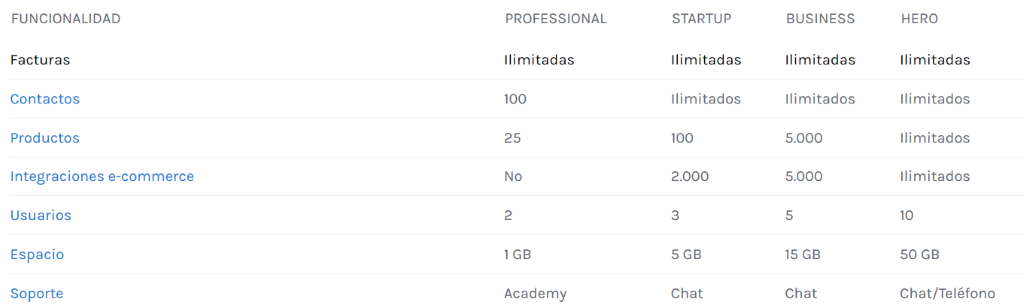
\includegraphics[scale=0.5]{images/func1.png}
\end{center}
\begin{itemize}
\item Idiomas: No especificado. 
\item Perfiles de usuario: Adaptado y personalizable. 
\item Personalización: Bastante personalizable.
\end{itemize}
\item \textbf{Sistema de soporte:}
\begin{itemize}
\item Diagnóstico de errores: No hay información. 
\item Solución de errores: Eficiente.         
\item Disponibilidad: Depende de la versión es más disponible o menos. Pero tiene buena disponibilidad. 
\item Actualizaciones : No hay información.
\end{itemize}
\item \textbf{Guía del Sistema:}
\begin{itemize}
\item Búsqueda de soluciones/dudas: Academy (Buscador, interacción entre usuarios y desarrolladores, publicación de soluciones). 
\item FAQ: Academy
\end{itemize}
\item \textbf{Accesibilidad:}
\begin{itemize}
\item Limitaciones físico/sensoriales: No existe. 
\item Limitaciones tecnológicas:  Se puede usar en cualquier dispositivo. 
\end{itemize}
\item \textbf{Coste:} Si elegimos la versión que pueden usar 5 usuarios (un usuario por departamento), serían 50 euros al mes, con pago anual.
\item \textbf{Casos de éxito:} Tres empresas, visionario, crepes y Texas y Verse
\end{itemize}
\item SugarCRM
\begin{itemize}
\item \textbf{Dashboard:} 
\begin{itemize}
\item Organización: La dashboard muestra la información de manera organizada, aunque no tiene muchas novedades. Es parecida a los demás CRMS.  
\end{itemize}
\item \textbf{Obtención de los datos:}
\begin{itemize}
\item Coherencia: Como los demás CRMs, tiene herramientas para importar y tratar esos datos importados, mediante archivos o Bases de Datos, etc. Aunque también se puede crear una BD nueva. 
\end{itemize}
\item \textbf{Procesamiento de datos:}
\begin{itemize}
\item Tratamiento de la ambigüedad:  Ninguna característica relevante, tratado por la herramienta BD que esté por debajo. 
\item Precisión: Suficiente. 
\item Integridad: Sin información suficiente.
\end{itemize}
\item \textbf{Tratamiento de la información:}
\begin{itemize}
\item Creación de documentos: A partir de la BD crea los documentos que se necesiten. 
\item Integración con BD existente: Bueno.
\end{itemize}
\item \textbf{Funcionalidad:}
\begin{itemize}
\item Idiomas: Existen módulos para añadir idiomas a la plataforma. 
\item Perfiles de usuario: Gran posibilidad de personalización de perfiles. 
\item Personalización: Muy  personalizable. 
\end{itemize}
\item \textbf{Sistema de soporte:}
\begin{itemize}
\item Diagnóstico de errores: Hay un soporte de usuario al cual se puede contactar y diagnosticarán el error, si existe. 
\item Solución de errores: Hay un soporte de ayuda para solucionar el problema.   
\item Disponibilidad: Buena disponibilidad durante las horas activas de la empresa. 
\item Actualizaciones : Cada x tiempo hay una actualización del CRM. 
\end{itemize}
\item \textbf{Guía del Sistema:}
\begin{itemize}
\item Búsqueda de soluciones/dudas: Existe una página de soporte con una guía de usuario y dudas resueltas. Y una comunidad de suaurios. 
\item FAQ: Disponible.
\end{itemize}
\item \textbf{Accesibilidad:}
\begin{itemize}
\item Limitaciones físico/sensoriales: Sin información. 
\item Limitaciones tecnológicas:  Multiplataforma. 
\end{itemize}
\begin{center}
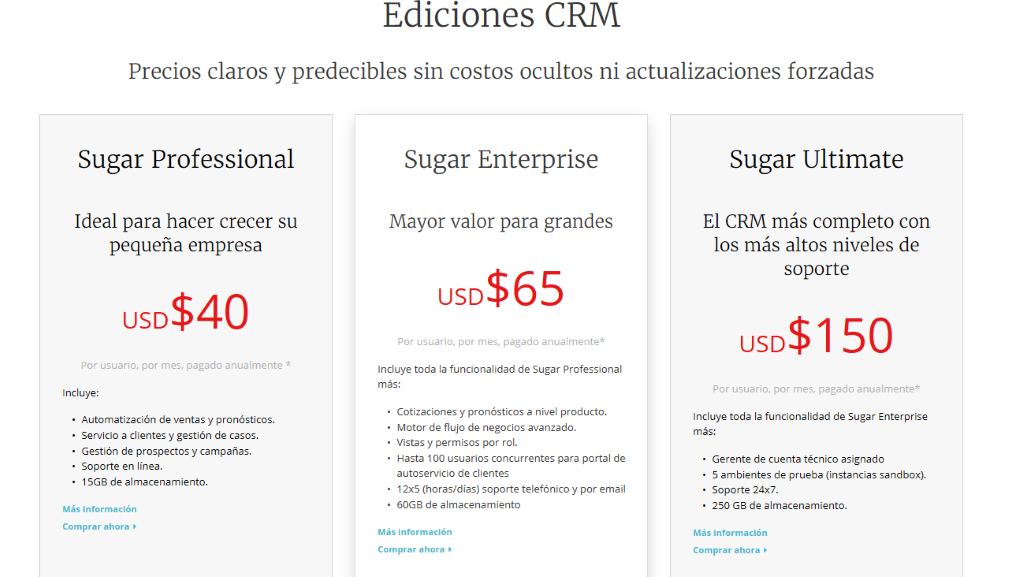
\includegraphics[scale=0.5]{images/coste.png}
\end{center}
\item \textbf{Coste:} Nuestra empresa con la versión profesional estaría bien. El coste sería de 35 euros por usuario y por mes, pagado anualmente. Bastante más alto que Holder CRM.
\item \textbf{Casos de éxito:} IBM, Uship.
\end{itemize}
\item Microsoft Dynamics CRM
\begin{itemize}
\item \textbf{Dashboard:}
\begin{center}
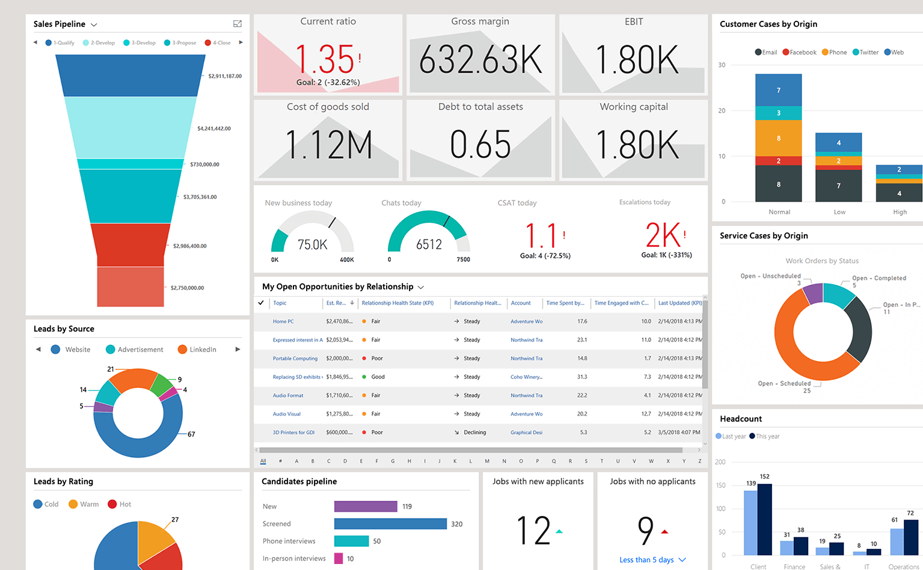
\includegraphics[scale=0.5]{images/dashboard.png}
\end{center}
\begin{itemize}
\item Organización: La dashboard de este CRM es similar a las demás, aunque la organización es un poco más intuitiva. 
\end{itemize}
\item \textbf{Obtención de los datos:}
\begin{itemize}
\item Coherencia: Existen herramientas que permiten importar datos de manera coherente, como son Import data Wizard. 
\end{itemize}
\item \textbf{Procesamiento de datos:}
\begin{itemize}
\item Tratamiento de la ambigüedad: Normal, ninguna característica relevante para este problema. 
\item Precisión: Suficiente. 
\item Integridad: Integridad con todos los software de Microsoft (Outlook, Windows 10, etc).
\end{itemize}
\item \textbf{Tratamiento de la información:}
\begin{itemize}
\item Creación de documentos: Genera los documentos que se necesiten en formato PDF. 
\item Integración con BD existente: Bueno.
\end{itemize}
\item \textbf{Funcionalidad:}
\begin{itemize}
\item Idiomas: Se pueden habilitar los paquetes de idiomas. 
\item Perfiles de usuario: Posibilidad de crear usuarios con distintos roles. 
\item Personalización: Se puede personalizar. 
\end{itemize}
\item \textbf{Sistema de soporte:}
\begin{itemize}
\item Diagnóstico de errores: Hay un sistema de soporte al que se le pueden poner tickets y ellos miran el problema o se puede contactar directamente con ellos. 
\item Solución de errores: En el momento en el que los técnicos del sistema de soporte leen el ticket o reciben una consulta, se encargan de solucionar el problema.          
\item Disponibilidad: Buena disponibilidad durante el horario activo de la empresa. 
\item Actualizaciones : Actualizaciones periódicas. 
\end{itemize}
\item \textbf{Guía del Sistema:}
\begin{itemize}
\item Búsqueda de soluciones/dudas: Hay un foro en el que se pueden preguntar dudas o buscar dudas resueltas. 
\item FAQ: Existe un foro con preguntas frecuentes bastante completo. 
\end{itemize}
\item \textbf{Accesibilidad:}
\begin{itemize}
\item Limitaciones físico/sensoriales: Tiene control para las discapacidades (como métodos abreviados de teclado) en temas de accesibilidad. 
\item Limitaciones tecnológicas: Multiplataforma, local, online. 
\end{itemize}
\item \textbf{Coste:} Al ser una empresa pequeña o mediana, con la versión básica de Microsoft Dinamics 365 valdría. Son 101€ por usuario y al mes, con pago anual, bastante más caros que las otras versiones analizadas. 
\begin{center}
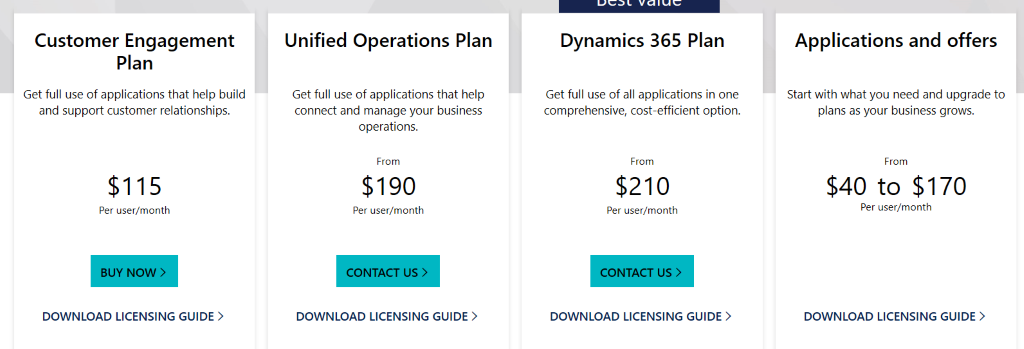
\includegraphics[scale=0.5]{images/costes.png}
\end{center}
\item \textbf{Casos de éxito:} Bastantes, entre ellos, Siemens, Fridays y Macys.
\end{itemize}
\end{itemize}

Los parámetros de ponderación escogidos han sido del 1 al 7, ya que hay un amplio abanico de criterios sobre los que calificar con distintas importancias. 

El modelo de calificación obtenido nos ha dado una calificación de 6950 para holder CRM, 7060 para Sugar CRM y 7980 para Microsoft Dynamics 365. Las calificaciones de los tres software han salido parecidas, pero finalmente la opción ganadora ha sido Microsoft Dynamics 365.

\begin{center}
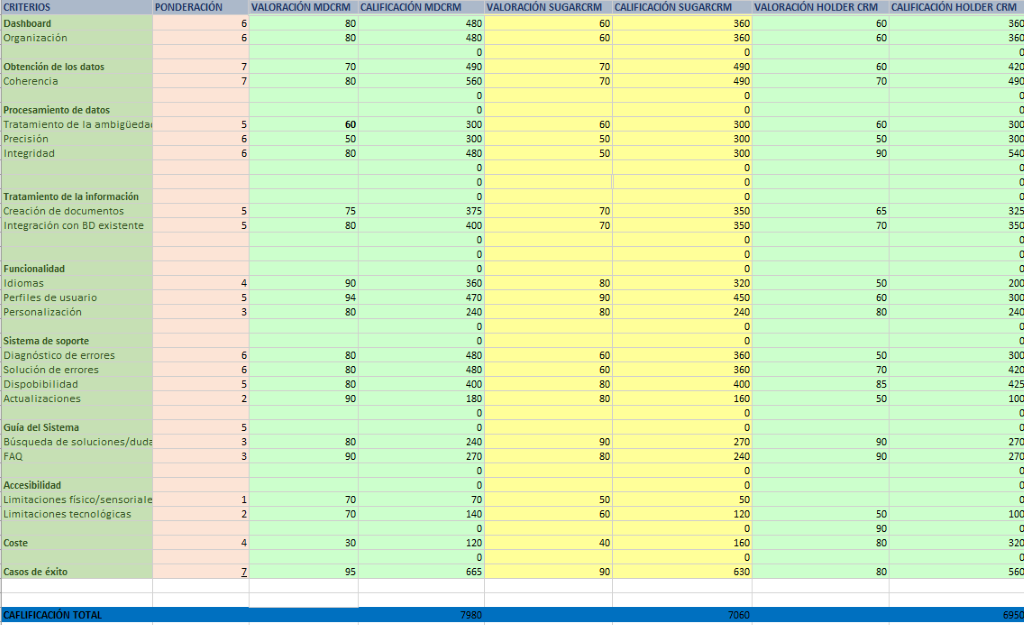
\includegraphics[scale=0.5]{images/ponderacion.png}
\end{center}

El modelo de calificación mostrado anteriormente se adjunta en formato “.excel” para futuras consultas o modificaciones. 

Para complementar la decisión de si adquirir un nuevo sistema de información o no, y en caso de implantarlo, elegir cuál, se ha creado un modelo de coste total de propiedad para calcular el coste a largo plazo de la implantación del nuevo software. 

\textbf{Coste total de propiedad}

\textbf{Criterios para calcular el coste de propiedad:}

\begin{center}
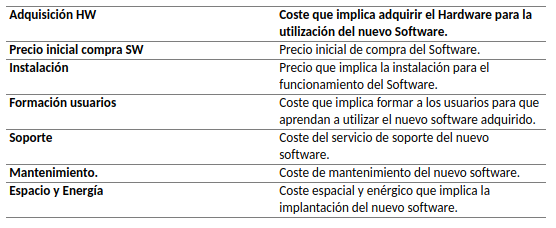
\includegraphics[scale=0.5]{images/costePropiedad.png}
\end{center}

\textbf{Calculo del Coste de la Propiedad}

\begin{center}
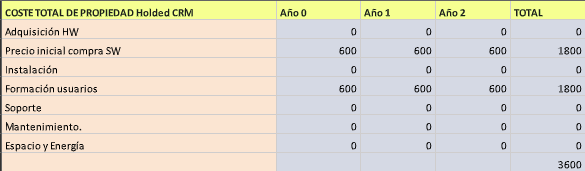
\includegraphics[scale=0.5]{images/Holded.png}
\end{center}

\begin{center}
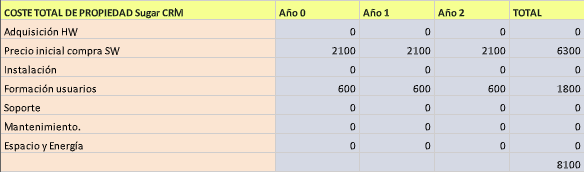
\includegraphics[scale=0.5]{images/sugar.png}
\end{center}

\begin{center}
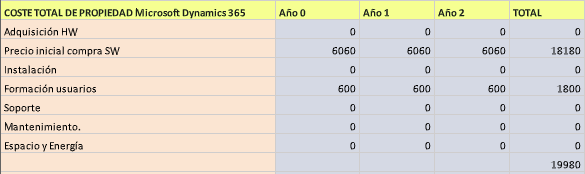
\includegraphics[scale=0.5]{images/Microsoft.png}
\end{center}

Observando los modelos de coste de propiedad creados, Microsoft Dynamics 365 es mucho más caro de los otros dos softwares. Holded CRM es notoriamente el más barato y Sugar CRM está en un lugar intermedio.

\vspace{5mm}

\textbf{\underline{Cambios que implicaría en la organización implantar la opción ganadora}}

\vspace{5mm}

Implantar la opción ganadora (Holder CRM)  implicaría un aumento en los gastos de la empresa a largo plazo, ya que las herramientas que se utilizan ahora, casi todas son de licencia libre y no tienen ningún coste. Aparte, cada departamento tiene ya su manera de trabajar y cambiar todos lod software por uno costaría tanto dinero, como tiempo y costaría volver a estabilizar el sistema de trabajo de la empresa.

\section{Sistemas de flujo de Trabajo}

\begin{itemize}
\item Identificar y modelar los principales flujos de trabajo de la empresa
\end{itemize}

Diagramas en Bizagi a modo explicativo de algunas funcionalidades que desempeña la empresa: 

\begin{itemize}
\item Renovar un cliente
\begin{center}
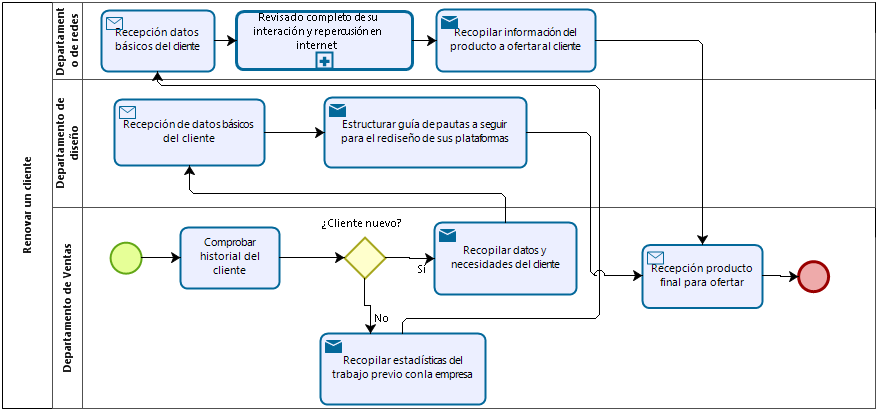
\includegraphics[scale=0.5]{images/cliente.png}
\end{center}
De manera sencilla podemos ver que el flujo de actividad de esta tarea la inicializa el departamento de ventas quien deberá llevar un historial de los posibles/futuros y actuales clientes, realizando actualizaciones periódicas sobre ellos (para ofrecerles nuevos productos o actualizar los que ya tengan). 

Dependiendo de si ya han trabajado previamente con la empresa o no, se recogerán todos los datos necesarios para generar los productos que necesite el cliente, en los márgenes y límites de tiempo establecidos y firmados mediante contratos.
\item Diseñar una página web
\begin{center}
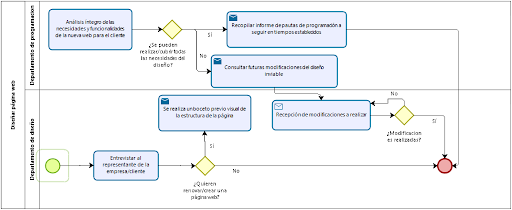
\includegraphics[scale=0.5]{images/web.png}
\end{center}
Para llevar acabo esta tarea será necesaria la comunicación entre el departamento de diseño y el departamento de programación, quiénes serán los encargados de dar el visto bueno final del proyecto. 

Primeramente, el Departamento de Diseño redactará una primera impresión de lo que será la página web que desee el cliente en función de una serie de entrevistas con él y de recopilar información. Una vez dicha información llegue al Departamento de Programación, ellos deberán ver si pueden poner en práctica, si es viable o tan siquiera si tiene sentido realizar todas las funcionalidades y maquetaciones que sugiere el Departamento de Diseño. Si todo funciona correctamente, se establecen los tiempos y fechas de entrega final y se daría comienzo a realizar dicha página, si por el contrario no fuera así, volvería el flujo de actividad sobre el Dpto. Diseño quién debería de rediseñar dicho proyecto para su óptimo funcionamiento.
\item Gestión de redes sociales
\begin{center}
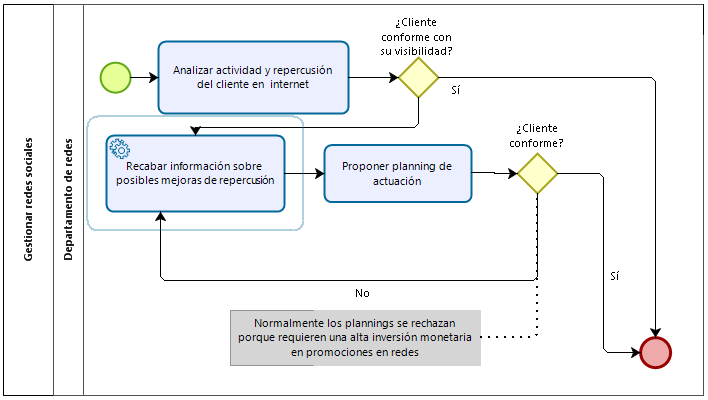
\includegraphics[scale=0.5]{images/rrss.png}
\end{center}
Dicho departamento se encargará de analizar mediante herramientas estadísticas y
promociones monetarias, la repercusión, el peso y el posicionamiento de las redes
de nuestro cliente. Si el cliente no está conforme con la situación actual, se le hará
un planning de actuación con respecto a la actividad que se programará para sus
redes, las promociones que tendrán y la repercusión que tendrá en base al público
que atraen, con el consecuente coste de llevar a cabo dicha campaña. Si el cliente lo
ve lógico y está conforme, dará paso al Dpto. A realizar dicha campaña, en caso
negativo, deberán crear un nuevo planning ó modificar el antíguo hasta lograr llegar
a un consenso.
\end{itemize}

\section{Propuestas innovadoras de Sistemas de Información para la Organización}

Utilizar menos software separados y usar uno solo para todos los departamentos.

\section{División de Tareas entre los miembros del grupo}

Para la repartición de tareas hemos creado una tabla:

\begin{center}
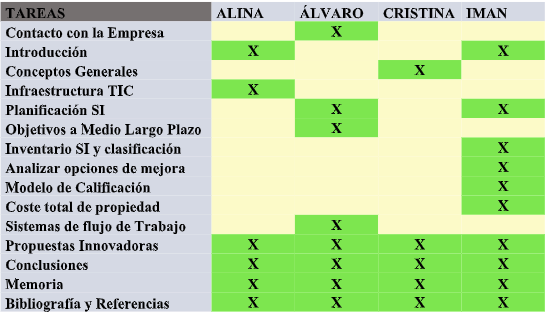
\includegraphics[scale=0.5]{images/tareas.png}
\end{center}

\section{Conclusión}

Al ser una empresa que ya tiene su sistema implantado y su propia manera de
trabajar, aunque analicemos mejoras que a largo plazo pueden mejorar el sistema
de la empresa en general, no se ve muy claro si realmente la empresa querría
implantarlo, ya que habría que conocer muy bien la duración media de los
trabajadores de la empresa y otros factores difíciles de conocer por personas
ajenas a la empresa.

\begin{thebibliography}{9}

\bibitem{SisDir} \textit{Sistema Directivo}, \url{https://blogs.udima.es/administracion-y-direccion-de-empresas/libros/introduccion-a-la-organizacion-de-empresas-2/unidad-didactica-2-el-sistema-de-direccion-y-organizacion-principios-y-modelos-organizativos/1-introduccion-concepto-y-estructura-del-sistema-directivo/}.
\bibitem{SisFis} \textit{Sistema Físico}, \url{https://es.slideshare.net/yadithmartinezlopez5/trabajo-yadith}.
\bibitem{SisInf} \textit{Sistema de información}, \url{https://es.wikipedia.org/wiki/Sistema_de_informaci\%C3\%B3n}.
\bibitem{Sol} \textit{Soluciones CRM}, \url{https://www.dynamics-crm.es/soluciones-crm}.
\bibitem{Trello} \textit{Trello}, \url{https://trello.com/?truid=trf9bee6-b868-4daa-8024-85319ae8cb44}.
\bibitem{FacBus} \textit{Facebook Business}, \url{https://business.facebook.com/}.
\bibitem{Ads} \textit{Google Ads}, \url{https://ads.google.com/intl/es_es/start/?subid=es-es-adon-bi-aw-c-0-r0_xx_txx_xx_xx_bau_non!o2~350070004-\%7bcreative\%7d-kwd-77446954221687:loc-170&sourceid=awo&utm_source=aw&utm_medium=ha&utm_campaign=es-es-adon-bi-aw-c-0-r0_xx_txx_xx_xx_bau_non!o2~350070004-\%7bcreative\%7d-kwd-77446954221687:loc-170&utm_term=Google\%20Ads&utm_content=Desk\%2BTab\%20\%7C\%20AW\%20SEM\%20\%7C\%20BKWS\%20\%7C\%20EXA\%20~\%20\%5BWE\%5D\%20ES_ES_EXA_R0_\%5B1\%3A1\%5D\%20google\%20ads_xx_xx_xx&gclid=CIGNwKq2pN8CFYaMhQodfcED2w}.
\bibitem{FacPix} \textit{Facebook Pixel}, \url{https://www.pixelsoftwares.com/}.
\bibitem{ImplCRM} \textit{Ejemplos de CRM}, \url{https://www.crmswitch.com/implementing-crm/six-crm-dashboard-examples/}.
\bibitem{Casos} \textit{Casos de éxito de Holded}, \url{https://www.holded.com/es/casos-de-exito-de-clientes-de-holded}.
\bibitem{SugarCRM} \textit{Sugar CRM}, \url{https://files.sugarcrm.com/resources/datasheets/sugar-professional-2016-05-20-es.pdf}.
\bibitem{Exportacion} \textit{Exportación de datos en Sugar CRM}, \url{http://www.tecnologiafacil.com/importacion-y-exportacion-masiva-de-datos-en-sugarcrm/}.
\bibitem{Winner} \textit{Business Choice Awards: CRM}, \url{http://sugarcrm-online.s3.amazonaws.com/misc/pcmag-business-choice-winner-2016-07-20.pdf}.
\bibitem{GesDoc} \textit{Gestión de documentos en Sugar CRM}, \url{https://www.connecting-software.com/gestion-de-documentos-sugarcrm-mas-efectiva/}.
\bibitem{Modulos} \textit{Modulos en Sugar CRM}, \url{http://rodriguezizquierdo.com/como-instalar-modulos-o-cambiar-idioma-en-sugarcrm-version-6-5-10-build-8716/}.
\bibitem{GesPro} \textit{Gestion de perfiles}, \url{https://bebeyond.es/gestion-de-perfiles-permisos-de-usuarios-crm/}.
\bibitem{SuppPlat} \textit{Plataformas soportadas por Sugar CRM}, \url{http://support.sugarcrm.com/Resources/Supported_Platforms/index.html}.
\bibitem{CasosExito} \textit{Casos de éxito de Sugar CRM}, \url{https://www.intelligencepartner.com/conoces-estos-casos-de-exito-con-sugarcrm/}.
\bibitem{DynamicCRM} \textit{How to Organize Dynamics CRM Documents in SharePoint}, \url{https://www.crmsoftwareblog.com/2018/02/organize-dynamics-crm-documents-sharepoint/}.
\bibitem{PaqIdioma} \textit{Instalar y habilitar un paquete de idioma}, \url{https://docs.microsoft.com/es-es/previous-versions/dynamicscrm-2016/deployment-administrators-guide/hh699736\%28v\%3dcrm.8\%29}.
\bibitem{Sec} \textit{Crear usuarios en Dynamics 365 (online) y asignar roles de seguridad}, \url{https://docs.microsoft.com/es-es/dynamics365/customer-engagement/admin/create-users-assign-online-security-roles}.
\bibitem{Supp} \textit{Soporte Dynamics 365}, \url{http://soportedynamics.com/servicios/soporte-dynamics-365/}.
\bibitem{Updates} \textit{Actualizaciones acumulativas para Microsoft Dynamics 365 local}, \url{https://support.microsoft.com/es-es/help/3142345/microsoft-dynamics-365-onpremise-cumulative-updates}.
\bibitem{FAQ} \textit{FAQ de la política de Actualización}, \url{https://docs.microsoft.com/en-us/dynamics365/get-started/faq-update-policy}.
\bibitem{Hist} \textit{Historias de clientes}, \url{https://dynamics.microsoft.com/es-es/customer-stories/}.

\end{thebibliography}

\end{document}